\chapter{State identification experiments}

\section{Introduction}

% TODO rewrite Chap. 1
As was pointed out in Chap. 1, the response of a nontrivial machine \emph{M} to specified excitations is unpredictable if the state of \emph{M} is unknown; this response, on the other hand, can always be predicted if the initial state is known. One of the basic tasks in the analysis of finite-state machines, therefore, is to identify the state of the machine under investigation. Once the state is identified, the behavior of the machine under all future conditions becomes determinable, and steps may be taken to force the machine into varios modes of operation desirable to the investigator.

    In this chapter we shall discuss two of the most important state identifications problems - that of identifying the initial state of a machine (i.e., the state in which a machine exists when presented to the investigator) and that of identifying the final state of a machine (i.e., the state in which a machine exists when the probing operations conducted by the investigator are completed). The solution to either of these problems constitutes the solution to the basic problem of rendering the machine predictable to the investigator. As will be seen in a later chapter, this solution is also useful in other problems, where the number of unknown quantities of interest is considerably larger than that involved in the state identification problem.

\section{Classification Experiments}

    The process of applying input sequences to the input terminals of a machine, observing the resulting output sequences, and drawing conclusions based on these observations will be called an \emph{experiment}. In all our discussions, without exception, it will be assumed that a machine on which an experiment is conducted is a sealed ``black box'' with only the input and output terminals accessible. Conclusions may be based only on applied excitations, observed responses, and possibly, on transition tables (or diagrams, or matrices) which may be available for the task at hand.

    We shall distinguish between two types of experiments:
\begin{enumerate}
    \item \emph{Preset experiments}, where the applied input sequence is completely determined in advance;
    \item \emph{Adaptive experiments}, where the applied input sequence is composed of two or more subsequences, each subsequence (except the first) determined on the basis of responses resulting from preceding subsequences.
\end{enumerate}

\begin{figure}
    \centering
    \begin{subfigure}{.85\textwidth}
        \centering
        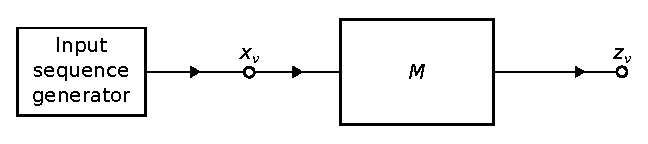
\includegraphics[width=256pt, clip]{images/eps/presetExperiment}
        \caption{Preset experiment}
        \qquad
    \end{subfigure}
    \begin{subfigure}{.85\textwidth}
        \centering
        \includegraphics[width=256pt, clip]{images/eps/adaptiveExperiment}
        \caption{Adaptive experiment}
    \end{subfigure}
    \caption{Types of experiments}
    \label{fig:experiments}
\end{figure}

    A preset experiment, as a rule, is easier to implement than an adaptive one: whereas the latter requires a number of intermediate decisions before the final decision is made, the former requires no such intermediate decisions. Envisioning a human or a mechanical ``input-sequence-generator'', whose function is to supply the machine with the required input sequences, it can be seen that in preset experiments the generator should be capable of supplying a single sequence only. In adaptive experiments, on the other hand, the generator should be capable of generating a number of sequences, each sequence based on information fed back from the output terminal of the machine. As we shall see, the advantage of some adaptive experiments is that they are relative concise; also, is some cases, adaptive experiments are easier to design than preset ones. A schematic representation of the two types of experiments is shown in Fig. \ref{fig:experiments}.

    One machine is referred to as the \emph{copy} of another machine, if both machines have identical transition tables, and if both are at the same state before the experiment commences. Experiments can be classified according to the number of copies which they require of the machine under investigation:

\begin{enumerate}
    \item \emph{Simple experiments}, where only one copy of the machine is required.
    \item \emph{Multiple experiments}, where more than one copy of the machine is required.
\end{enumerate}

    As most machines encountered in practice are available in one copy only, simple experiments are preferable to multiple ones.

    The \emph{length} of an experiment is taken as the total number of input symbols applied in the course of conducting the experiment. The \emph{order} of an experiment is taken as the number of input subsequences (i.e., sequences separated by decision-making operations) of which the experiment is composed. The \emph{multiplicity} of an experiment is the number of copies it requires of the machine under investigation. Thus, a preset experiment is an experiment of order 1, and an adaptive experiment is an experiment of order 2 or greater. A simple experiment is an experiment of multiplicity 1, and a multiple experiment is an experiment of multiplicity 2 or greater. The length, order, and multiplicity of an experiment may be regarded as rough measures of its execution cost.

\section{Diagnosing and Homing Experiments}

    Our main concern in this chapter is to devise experiments for solving the following two problems:
\begin{enumerate}
    \item \emph{The diagnosing problem}: It is knwon that a given machine \emph{M}, whose transition table is available, is in one of the states $ \sigma_{i_{1}}, \sigma_{i_{2}}, ..., \sigma_{i_{m}}  $. Find this state.

    \item \emph{The homing problem}: It is known that a given machine $M$, whose transition table is available, is in one of the states $\sigma_{i_{1}}, \sigma_{i_{2}}, ..., \sigma_{i_{m}}$. Pass $M$ into a known state.
\end{enumerate}


    The diagnosing problem, then, is that of identifying the initial state of $M$, and the homing problem os that of identifying the final state of $M$. An experiment which solves the diagnosing problem is called \emph{diagnosing experiment}; an experiment which solves the homing problem is called a \emph{homing experiment}. Clearly, every diagnosing experiment is also a homing experiment, since the knowledge of the initial state of $M$ and the applied sequence implies the knowledge of the final state. The converse, however, is not necessarily true.

    Unless otherwise specified, it will be assumed throughout this chapter that $M$ is a minimal machine. If $M$, as originally specified by its transition table, is not minimal, it can always be minimized by methods introduced in Chapter \ref{chapter:equivAndMinimization}. Since only the external behavior of $M$ is of interest, there is no risk in replacing the original table by that of the minimal form, and, hence, there is no loss in generality in assuming that $M$ is minimal.

    The set of states $\{ \sigma_{i_{1}}, \sigma_{i_{2}}, ..., \sigma_{i_{m}} \} $, one of which is, to the investigator's knowledge, the initial state of $M$, is called \emph{admissible set} of $M$ and denoted by $A(M)$. The states in $A(M)$ are called \emph{admissable states}. Both the diagnosing and homing problems are trivial when $A(M)$ is a singleton, i.e., when $\emph{m}=1$. Our atention, therefore, will concentrate on the cases where $m \geq 2$.

    It can be noted that preset diagnosing or homing experiments are indepedent of the true initial state of $M$. On the other hand, adaptative diagnosing or homing experiments depend, in general, on the true inital state of $M$. This follows from the fact that the initial state determines the response of $M$ to the first input subsequence; since the composition of the next input subsequence is based on the response of the currently applied subsequence, the initial state determines all input subsequences except the first.

\section{Pairwise Diagnosing Experiments}

    The problem of identifying the initial state of machine $M$ when $A(M)$ is of an arbitrary size of \emph{m} is inherently much more complex that that pertaining to the special case $ \emph{m} = 2 $. To differentiate between the general and the special problems, the former will be referred to as the \emph{m-wise diagnosing problem}, while the latter will be referred to as the \emph{pairwise diagnosing problem}.

    In this section we shall tackle the pairwise diagnosing problem, assuming that the given machine $M$ is an n-state machine, with $A(M) = \{ \sigma_{i_{0}}, \sigma_{j_{0}} \}$. Since $M$ is minimal, $\sigma_{i_{0}}$ and $\sigma_{j_{0}}$ must be distinguishable, and hence $(n-1)$-distinguishable. Consequently, there exists an input sequence of length $n-1$ or less which, when applied to $ M|\sigma_{i_{0}}$ and $ M|\sigma_{j_{0}}$ yields distinct output sequences. Such an input sequence is called a \emph{diagnosing sequence} for $ \{  \sigma_{i_{0}}, \sigma_{j_{0}} \} $. The pairwise diagnosing experiment for $M$ and 
\begin{equation*}
    A(M) = \{ \sigma_{i_{0}}, \sigma_{j_{0}} \} 
\end{equation*}
consists, therefore, of applying the diagnosing sequence for $ \{  \sigma_{i_{0}}, \sigma_{j_{0}} \} $ to $M$ and observing the response; on the basis of this response, the true initial state can be identified. In the remainder of this section we shall show how diagnosing sequences for specified pairs of states can be constructed. Let $\sigma_{i_{0}}$ and $\sigma_{j_{0}}$ be \emph{l}-distinguishable and $(\emph{l}-1)$-equivalent, for some $1 \leq \emph{l} \leq \emph{n}-1 $. Then the length of the shortest diagnosing sequence for $ \{  \sigma_{i_{0}}, \sigma_{j_{0}} \} $ is \emph{l}. Any diagnosing sequence for $ \{  \sigma_{i_{0}}, \sigma_{j_{0}} \} $ whose length is \emph{l}, as specified above, will be called a \emph{minimal diagnosing sequence} for $ \{  \sigma_{i_{0}}, \sigma_{j_{0}} \} $ and denoted by $ \upvarepsilon(\sigma_{i_{0}}, \sigma_{j_{0}} )  $. If $\sigma_{i_{0}}$ and $\sigma_{j_{0}}$ are \emph{l}-distinguishable and $(\emph{l}-1)$-equivalent, $\sigma_{i_{0}}$ and $\sigma_{j_{0}}$ must be disjoint states in $P_l$ and adoint $P_{l-1}$. \emph{l}, therefore, can be determined by constructing the \emph{k}-equivalence partitions for the given machine $M$ and noting the lowest value of \emph{k} such that $P_k$ contains $\sigma_{i_{0}}$ and $\sigma_{j_{0}}$  in two separate classes; this value must equal \emph{l}.

When $ \upvarepsilon(\sigma_{i_{0}}, \sigma_{j_{0}} ) $ is applied to $ M|\sigma_{i_{0}}$ and $ M|\sigma_{j_{0}}$, the output sequences are identical except for the very last - the \emph{l}th - symbol. Consequently, the \emph{k}th successors of $\sigma_{i_{0}}$ and $\sigma_{j_{0}}$, with respect to $ \upvarepsilon(\sigma_{i_{0}}, \sigma_{j_{0}} ) $ are $ (\emph{l} - \emph{k})$-distinguishable and $(\emph{l} - \emph{k} - 1)$-equivalent, for all $0 \leq \emph{k} \leq \emph{l}-1 $. This situation is depicted in Fig. \ref{fig:minimalDiagSequence}, where $ \upvarepsilon(\sigma_{i_{0}}, \sigma_{j_{0}} ) $  is taken as $\xi_{u_{1}}\xi_{u_{2}}...\xi_{u_{l}}$

\begin{figure}
    \centering
    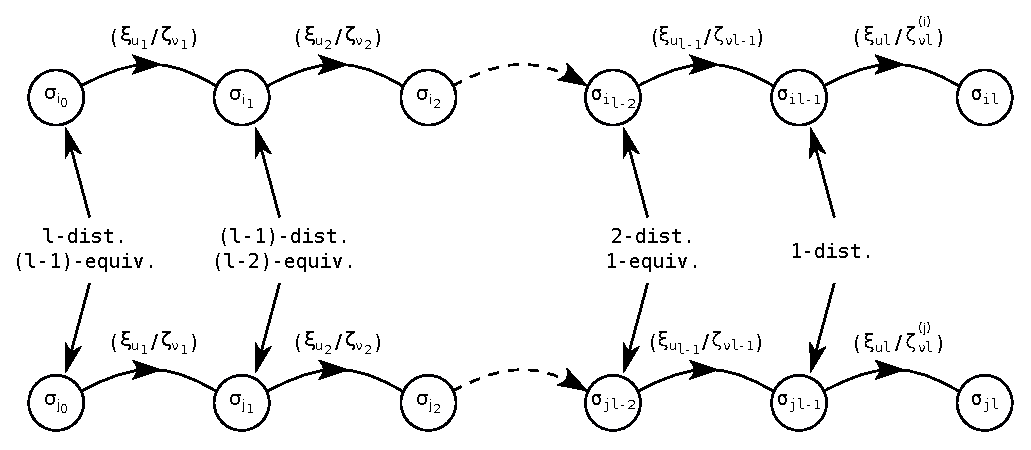
\includegraphics[width=330pt,clip]{images/eps/minimalDiagnosingSequence}
    \caption{Minimal diagnosing sequence for $\{ \sigma_{i_{0}}, \sigma_{j_{0}} \}$ }
    \label{fig:minimalDiagSequence}
\end{figure}

The sequence of states traversed by $ M|\sigma_{i_{0}}$ is $\sigma_{i_{1}}, \sigma_{i_{2}}, ..., \sigma_{i_{l}} $, the sequence of states traversed by $ M|\sigma_{j_{0}} $ is $\sigma_{j_{1}}, \sigma_{j_{2}}, ..., \sigma_{j_{l}} $, the output sequence yield by $ M|\sigma_{i_{0}}$ is $\zeta_{\nu_{1}}, \zeta_{\nu_{2}}, ..., \zeta^{(i)}_{\nu_{l}} $ and the output sequence yielded by $ M|\sigma_{j_{0}} $ is $\zeta_{\nu_{1}}, \zeta_{\nu_{2}}, ..., \zeta^{(j)}_{\nu_{l}} $ where $ \zeta^{(i)}_{\nu_{l}} \neq \zeta^{(j)}_{\nu_{l}} $. Using the notation of Fig. \ref{fig:minimalDiagSequence}, it can be stated that, if $\sigma_{i_{0}}$ and $\sigma_{j_{0}}$ are \emph{l}-distinguishable and $(\emph{l}-1)$-equivalent, and if $\xi_{u_{1}}\xi_{u_{2}}...\xi_{u_{l}}$ is a minimal diagnosing sequence for $\{  \sigma_{i_{0}}, \sigma_{j_{0}}\}$, then: \begin{inparaenum}[(1) ]
    \item For $ 1 \leq \emph{k} \leq \emph{l} - 1$, $\xi_{u_{k}}$ is an input symbol which passed $\sigma_{i_{k-1}}$ and $\sigma_{j_{k-1}}$ into a pair of $(\emph{l} - \emph{k})$-distinguishable and $(\emph{l} - \emph{k} - 1)$-equivalent states $\sigma_{i_{k}}$ and $\sigma_{j_{k}}$.
    \item $\xi_{u_{l}}$ is an inpu symbol which yields distinct output symbols when applied to $ M|\sigma_{i_{l-1}}$ and $ M|\sigma_{j_{l-1}}$.
\end{inparaenum}

\emph{Determining $\xi_{u_{k}}$, $\sigma_{i_{k}}$, and  $\sigma_{j_{k}}$ from $\sigma_{i_{k-1}}$ and $\sigma_{j_{k-1}}$ } $(1 \leq \emph{k} \leq \emph{l} - 1)$. The determination of $\xi_{u_{k}}$, $\sigma_{i_{k}}$, and  $\sigma_{j_{k}}$ when $\sigma_{i_{k-1}}$ and $\sigma_{j_{k-1}}$ are known can be most conveniently carried out with the aid of the $P_k$ tables, whose construction for the equivalence partitioning of a given machine is described in Sec. \ref{section:partitionByPkTables}. $\sigma_{i_{k-1}}$ and $\sigma_{j_{k-1}}$ are $(\emph{l} - \emph{k} + 1)$-distinguishable and $(\emph{l}-\emph{k})$-equivalent states; consequently, they constitute adjoint rows in the $P_{l-k}$ table and disjoint rows in the $P_{l-k+1}$ table. Rows $\sigma_{i_{k-1}}$ and $\sigma_{j_{k-1}}$ in the $P_{l-k}$ table must, therefore exhibit two entries, say $\sigma^{'}_{i_{k-1}}$ and $\sigma^{'}_{j_{k-1}}$, respectively, which have different subscripts in at least one column, say $\xi^{'}_{u_{k-1}}$. Now $\sigma^{'}_{i_{k-1}}$ and $\sigma^{'}_{j_{k-1}}$ must be $(\emph{l}-\emph{k}-1)$-equivalent, since they are first successors of the  $(\emph{l}-\emph{k})$-equivalent states $\sigma_{i_{k-1}}$ and $\sigma_{j_{k-1}}$, with respect to the input symbol $\xi^{'}_{u_{k-1}}$; they also must be $(\emph{l} - \emph{k})$-distinguishable, since ``$\sigma^{'}_{i_{k-1}}$'' and ``$\sigma^{'}_{j_{k-1}}$'' bear different subscripts in the $P_{l-k}$ table. Consequently, $\sigma^{'}_{i_{k-1}}$ and $\sigma^{'}_{j_{k-1}}$ are the sought states $\sigma_{i_{k}}$, and  $\sigma_{j_{k}}$, respectively, and the input symbol $\xi^{'}_{u_{k-1}}$ is the sought input symbol $\xi_{u_{k}}$. Thus, $\xi_{u_{k}}$, $\sigma_{i_{k}}$, and  $\sigma_{j_{k}}$ can be determined by inspection of the $P_{l-k}$ table.

\emph{Determining $ \xi_{u_{l}}$ from $\sigma_{i_{l-1}}$ and $\sigma_{j_{l-1} }$}. $\sigma_{i_{l-1}}$ and $\sigma_{j_{l-1}}$ are \emph{l}-distinguishable; hence, there must exist at least one input symbol which yields distinct output symbols when applied to $ M|\sigma_{i_{l-1}}$ and $ M|\sigma_{j_{l-1}}$. This symbol , which is the sought $\xi_{u_{l}}$ can be readily determined by locating a column in the $z_\nu$ subtable, in which rows $\sigma_{i_{l-1}}$ and $\sigma_{j_{l-1}}$ have distinct entries.

    The foregoing procedure can now be combined as follows:

\algorithm $\sigma_{i_{0}}$ and $\sigma_{j_{0}}$ are two states in machine $M$. To determine the minimal diagnosing sequence for $ \{  \sigma_{i_{0}}, \sigma_{j_{0}} \} $:  \begin{inparaenum}[ (1) ]
    \item Construct the $P_k$ tables for $M$. Find \emph{l} such that $\sigma_{i_{0}}$ and $\sigma_{j_{0}}$ are adjoint rows in the $P_{l-1}$ table and disjoint rows in the $P_l$ table. Let $\emph{k}=1$.
    \item \begin{inparaenum}[ (a) ]
        \item If $ \emph{l} - \emph{k} > 0 $, proceed to step 3.
        \item If $ \emph{l} - \emph{k} = 0 $, $\xi_{u_{k}}$ is given by the heading of any column in the $z_\nu$ subtable of $M$, such that rows $\sigma_{i_{k-1}}$ and $\sigma_{j_{k-1}}$ in this column are distinct. $\xi_{u_{1}}\xi_{u_{2}}...\xi_{u_{k}}$ is the minimal diagnosing sequence for $ \{  \sigma_{i_{0}}, \sigma_{j_{0}} \} $.
    \end{inparaenum}
\item $\xi_{u_{k}}$ is the heading of any column in the $P_{l-k}$ table of $M$, such that rows $\sigma_{i_{k-1}}$ and $\sigma_{j_{k-1}}$ in this column have differently subscripted entries, these entries are $\sigma_{i_{k}}$, and  $\sigma_{j_{k}}$, respectively. Increment \emph{k} by 1 and return to (2).
\end{inparaenum}

    % TODO:  add figure 4.3
    %TODO: remove to keep \incSampleMachine in the future
    \setcounter{machineNumber}{16}
    \incSampleMachine
    Machine \sampleMachine \label{labelMachineA17} of Fig. \ref{fig:machineA17}  and Table \ref{table:deltaTableA17} will be used for illustration. Tables \ref{table:tableP1A17} to \ref{table:tableP4A17} are the $P_1, P_2, P_3$ and $P_4$ tables of \ref{labelMachineA17}. For example, to find the minimal diagnosing sequence for $\{1,2\}$, namely $ \upvarepsilon( 1, 2 )$, we start from $P_3$ table, which is the ``last'' table in which rows 1 and 2 are adjoint. Rows 1 and 2 in the $P_3$ table have distinct subscripts in entries ``$4_c$'' and ``$5_d$'' which appear in column $\beta$. $\beta$, then, is the first symbol in $\upvarepsilon(1,2)$. In the $P_2$ table, rows 4 and 5 have distinct subscripts in entries ``$3_b$'' and ``$2_a$'' which appears in column $\alpha$. $\alpha$, then, is the second symbol in $\upvarepsilon(1,2)$. In the $P_1$ table, rows 3 and 2 have distinct subscripts in entries ``$5_b$'' and ``$1_a$'', which appears in column $\alpha$. $\alpha$, then, is the third symbol in $\upvarepsilon(1,2)$. Alternatively, $\beta$ could be chosen as the third symbol, since rows 3 and 2 have distinct subscripts in entries ``$1_a$'' and ``$5_b$'',  which appear in column $\beta$. In the $z_\nu$ subtable, rows 1 and 5 have distinct entries (0 and 1) in column $\alpha$. $\alpha$, then, is the fourth and last symbol in $\upvarepsilon(1,2)$. Thus, (1,2) is either $\beta\alpha\alpha\alpha$ or $\beta\alpha\beta\alpha$.
\begin{figure}[h]
    \centering
    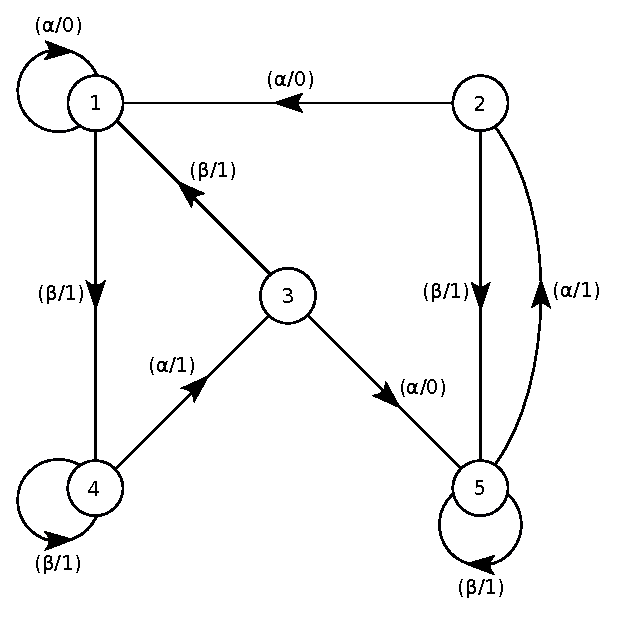
\includegraphics[width=220pt,clip]{images/eps/machineA17}
    \caption{Machine \ref{labelMachineA17}}
    \label{fig:machineA17}
\end{figure}
 From Table \ref{table:deltaTableA17} or Fig. \ref{fig:machineA17} it can be readily verified that when $\beta\alpha\alpha\alpha$ is applied to \ref{labelMachineA17} at state 1 and state 2, the last output symbol is 1 and 0, respectively. Consequently, if $\{1,2\}$ is the admissable set of \ref{labelMachineA17}, the diagnosing experiment may be conducted by applying $\beta\alpha\alpha\alpha$ and observing the last input: if this symbol is 1, the initial state is 1, and if this symbol is 0, the initial state is 2. Table \ref{table:diagSequenceA17} lists the minimal diagnosing sequences for all pairs of states $ \{  \sigma_{i_{0}}, \sigma_{j_{0}} \} $ in \ref{labelMachineA17}; the last two columns in this table indicate the last output symbols $\zeta^{(i)}_{\nu_{l}}$ and $\zeta^{(j)}_{\nu_{l}}$ observed when the minimal diagnosing sequence is applied to $\sigma_{i_{0}}$ and $\sigma_{j_{0}}$, respectively. Where two or more minimal diagnosing sequences can be constructed for a given state pair, only one such sequence is listed in the table.

\begin{table}[h]
\parbox{ .45\linewidth }{
    \centering
    \begin{tabular}{ c |c | c  | c | c  }
        \cline{2-5} &  \multicolumn{2}{ c |}{ $z_\nu$ } & \multicolumn{2}{c}{ $s_{\nu+1}$ } \\
        \hline 
        \multicolumn{1}{c|}{  \backslashbox{$s_\nu$}{ $x_{\nu}$  } } & $\alpha$ & $\beta$ & $\alpha$ & $\beta$ \\
        \hline
        1 & 0 & 1 & 1 & 4 \\
        2 & 0 & 1 & 1 & 5 \\
        3 & 0 & 1 & 5 & 1 \\
        4 & 1 & 1 & 3 & 4 \\
        5 & 1 & 1 & 2 & 5 \\
        \hline
    \end{tabular}
    \caption{ Machine \ref{labelMachineA17} }
    \label{table:deltaTableA17}
}
\qquad
\parbox{ .45\linewidth }{
    \centering
    \begin{tabular}{ cc | c | c }
        \cline{3-4} & & \multicolumn{2}{c}{ $s_{\nu+1}$ } \\
        \hline
        \multicolumn{1}{c|}{ $ \Sigma $ } & \backslashbox{$s_\nu$}{ $x_{\nu}$  } & $\alpha$ & $\beta$ \\
        \hline
        \multicolumn{1}{c|}{ \multirow{3}{*}{a}}  & 1 & $1_a$ & $4_b$ \\
        \multicolumn{1}{c|}{}                     & 2 & $1_a$ & $5_b$ \\
        \multicolumn{1}{c|}{}                     & 3 & $5_b$ & $1_a$ \\
        \hline
        \multicolumn{1}{c|}{ \multirow{2}{*}{b}}  & 4 & $3_a$ & $4_b$ \\
        \multicolumn{1}{c|}{}                     & 5 & $2_a$ & $5_b$ \\
        \hline
    \end{tabular}
    \caption{ $P_1$ Table for \ref{labelMachineA17} }
    \label{table:tableP1A17}
}
\end{table}

\begin{table}[h]
\parbox{ .45\linewidth }{
    \centering
    \begin{tabular}{ cc | c | c }
        \cline{3-4} & & \multicolumn{2}{c}{ $s_{\nu+1}$ } \\
        \hline
        \multicolumn{1}{c|}{ $ \Sigma $ } & \backslashbox{$s_\nu$}{ $x_{\nu}$  } & $\alpha$ & $\beta$ \\
        \hline
        \multicolumn{1}{c|}{ \multirow{2}{*}{a}}  & 1 & $1_a$ & $4_c$ \\
        \multicolumn{1}{c|}{}                     & 2 & $1_a$ & $5_c$ \\
        \hline
        \multicolumn{1}{c|}{ \multirow{1}{*}{b}}  & 3 & $5_c$ & $1_a$ \\
        \hline
        \multicolumn{1}{c|}{ \multirow{2}{*}{c}}  & 4 & $3_b$ & $4_c$ \\
        \multicolumn{1}{c|}{}                     & 5 & $2_a$ & $5_c$ \\
        \hline
    \end{tabular}
    \caption{ $P_2$ Table for \ref{labelMachineA17} }
    \label{table:tableP2A17}
}
\qquad
\parbox{ .45\linewidth }{
    \centering
    \begin{tabular}{ cc | c | c }
        \cline{3-4} & & \multicolumn{2}{c}{ $s_{\nu+1}$ } \\
        \hline
        \multicolumn{1}{c|}{ $ \Sigma $ } & \backslashbox{$s_\nu$}{ $x_{\nu}$  } & $\alpha$ & $\beta$ \\
        \hline
        \multicolumn{1}{c|}{ \multirow{2}{*}{a}}  & 1 & $1_a$ & $4_c$ \\
        \multicolumn{1}{c|}{}                     & 2 & $1_a$ & $5_d$ \\
        \hline
        \multicolumn{1}{c|}{ \multirow{1}{*}{b}}  & 3 & $5_d$ & $1_a$ \\
        \hline
        \multicolumn{1}{c|}{ \multirow{1}{*}{c}}  & 4 & $3_b$ & $4_c$ \\
        \hline
        \multicolumn{1}{c|}{ \multirow{1}{*}{d}}  & 5 & $2_a$ & $5_d$ \\
        \hline
    \end{tabular}
    \caption{ $P_3$ Table for \ref{labelMachineA17} }
    \label{table:tableP3A17}
}
\end{table}

\begin{table}[h]
    \centering
    \begin{tabular}{ cc | c | c }
        \cline{3-4} & & \multicolumn{2}{c}{ $s_{\nu+1}$ } \\
        \hline
        \multicolumn{1}{c|}{ $ \Sigma $ } & \backslashbox{$s_\nu$}{ $x_{\nu}$  } & $\alpha$ & $\beta$ \\
        \hline
        \multicolumn{1}{c|}{ \multirow{1}{*}{a}}  & 1 & $1_a$ & $4_d$ \\
        \hline
        \multicolumn{1}{c|}{ \multirow{1}{*}{b}}  & 2 & $1_a$ & $5_e$ \\
        \hline
        \multicolumn{1}{c|}{ \multirow{1}{*}{c}}  & 3 & $5_e$ & $1_a$ \\
        \hline
        \multicolumn{1}{c|}{ \multirow{1}{*}{d}}  & 4 & $3_c$ & $4_d$ \\
        \hline
        \multicolumn{1}{c|}{ \multirow{1}{*}{e}}  & 5 & $2_b$ & $5_e$ \\
        \hline
    \end{tabular}
    \caption{ $P_4$ Table for \ref{labelMachineA17} }
    \label{table:tableP4A17}
\end{table}

\begin{table}[t]
    \centering
    \begin{tabular}{ c | c | c | c | c }
        \hline
        $\sigma_{i_{0}}$ & $\sigma_{j_{0}}$ & $\upvarepsilon(\sigma_{i_{0}}, \sigma_{j_{0}}) $ & $\zeta^{(i)}_{\nu_{l}}$ & $\zeta^{(j)}_{\nu_{l}}$ \\
        \hline
        1 & 2 & $\beta\alpha\alpha\alpha $ & 1 & 0 \\
        1 & 3 & $\alpha\alpha$ & 0 & 1 \\
        1 & 4 & $\alpha$ & 0 & 1 \\
        1 & 5 & $\alpha$ & 0 & 1 \\
        2 & 3 & $\alpha\alpha$ & 0 & 1 \\
        2 & 4 & $\alpha$ & 0 & 1 \\
        2 & 5 & $\alpha$ & 0 & 1 \\
        3 & 4 & $\alpha$ & 0 & 1 \\
        3 & 5 & $\alpha$ & 0 & 1 \\
        4 & 5 & $\alpha\alpha\alpha $ & 1 & 0 \\
        \hline
    \end{tabular}
    \caption{Minimal Diagnosing Sequence for State Pairs in \ref{labelMachineA17}}
    \label{table:diagSequenceA17}
\end{table}


%$\xi_{u_{k}}$
%$\xi^{'}_{u_{k}}$
%$\sigma_{i_{k}}$, and  $\sigma_{j_{k}}$
%$\sigma_{i_{k-1}}$ and $\sigma_{j_{k-1}}$
%$\sigma^{'}_{i_{k-1}}$ and $\sigma^{'}_{j_{k-1}}$
%
%$(\emph{l} - \emph{k})$-distinguishable
%$(\emph{l}-\emph{k}-1)$-equivalent
%
%$\sigma_{i_{0}}$ and $\sigma_{j_{0}}$
%$ M|\sigma_{i_{0}}$ and $ M|\sigma_{j_{0}}$, 
%$ \{  \sigma_{i_{0}}, \sigma_{j_{0}} \} $
%$\zeta_{\nu_{0}}, \zeta_{\nu_{1}}, ..., \zeta^{(i)}_{\nu_{l}} $
%$\xi_{u_{1}}\xi_{u_{2}}...\xi_{u_{l}}$

